\documentclass{article}

\usepackage{amssymb,amstext,amsmath,graphicx,float,subfig,array,hyperref}
\usepackage[hmargin=3cm,vmargin=3.5cm]{geometry}

\begin{document}

\title{Preliminary Report for Orbital Design for a Lunar Impact
  Mission}
\author{Ricardo Medina}
\date{\today}

\maketitle
\thispagestyle{empty}
\pagebreak

\noindent
\small{\LaTeX}

\section{Free Body Diagrams and Equations of Motion}
\label{sec:motion}
The force due to the earth's gravity on a body in space is:
\begin{equation}
  \vec{F} = -\frac{GM_em}{r^2}\frac{\vec{r}}{r} =
  -\frac{GM_em}{r^3}\langle x, \; y, \; z \rangle = m\vec{a},
\end{equation}
where $m$ is the mass of the body orbiting the earth, $M_e$ is the
mass of the earth, $r$ is the distance from the center of the earth to
the body, and $\vec{r} = \langle x, \; y, \; z \rangle$ is the position vector
of the body with $i, j,$ and $k$ components. Thus:
\begin{align}
  -\frac{GM_em}{r^3}\langle x \; y \; z \rangle &= m\langle \frac{d^2x}{dt}, \;
  \frac{d^2y}{dt}, \;  \frac{d^2z}{dt} \rangle \intertext{and} \\
  \therefore \; -\frac{GM_e}{r^3}\langle x \; y \; z \rangle &= \langle \frac{d^2x}{dt}, \;
  \frac{d^2y}{dt}, \;  \frac{d^2z}{dt} \rangle.
\end{align}

Matlab, however, does not take second-order differential equations, so
the first derivatives are needed as well in the array that gets
passed to MatLab's differential equation solver:
\begin{equation}
  \frac{d}{dt}
  \begin{bmatrix}
    x \\ y \\ z \\ v_x \\ v_y \\ v_z
  \end{bmatrix} =
  \begin{bmatrix}
    v_x \\ v_y \\ v_z \\
    -GM_ex/r^3 \\
    -GM_ey/r^3 \\
    -GM_ez/r^3
  \end{bmatrix}
  \label{eq:eom}  
\end{equation}.
From this, it is clear that initial values for $x, y, z, v_x, v_y,
v_z$ are needed in order to get usable result. For the satellite, we
are assuming that it starts at perigee, and for the sake of plotting
the moon, the same will be assumed.

\section{Satellite Orbit Background}

As stated in A.2, data about satellite orbit, in particular ARIANE
GTO, comes as 5 pieces of information: inclination, $\theta$, altitude of
periapsis, $r_p$, altitude of apoapsis, $r_a$, longitude of first
ascending node, $\Omega$, and the argument of the periapsis, $\omega$.

According to A.6, these values are: \\
\begin{tabular}{|l|c|}
  \hline
  Inclination & 7 degrees \\ \hline
  Altitude of perigee & 250 km \\ \hline
  Altitude of apogee & 35950 km\\ \hline
  Argument of perigee & 178 degrees \\ \hline
  Longitude of first ascending node & 180 degrees \\ 
  \hline
\end{tabular}
\bigskip

\noindent
The equations for position and velocity of the satellite at
perigee are given as:
\begin{align}
  \vec{r_p} &= r_p  \langle
  (\cos{\omega}\cos{\Omega}-\sin{\omega}\cos{\theta}), \;
  (\cos{\omega}\sin{\Omega}+\sin{\omega}\cos{\Omega}\cos{\theta}), \;
  (\sin{\omega}\sin{\omega}) \rangle \\
  \vec{v_p} &= (2\mu\frac{r_a}{r_p(r_a+r_p)})^{\frac{1}{2}}
  \langle
  -(\sin{\omega}\cos{\Omega}+\cos{\omega}\sin{\Omega}\cos{\theta}),
  \;
  (\cos{\omega}\cos{\Omega}\cos{\theta}-\sin{\omega}\sin{\Omega}),
  \;
  (\cos{\omega}\sin{\theta})
  \rangle,
\end{align}
where $\vec{r_p}$ is the position vector of the satellite at perigee,
$\vec{v_p}$ is the velocity vector of the satellite at perigee,
and $\mu$ is a gravitational parameter that is the product of the
gravitational constant and the mass of the earth. Simply plugging into
a function in Matlab would give the initial conditions for the
satellite.

A function called \verb[satellite[ that takes 7 parameters (the five
orbit parameters, the radius of the body its orbiting, and the
gravitational parameter) outputs the initial
position and velocity of the satellite as well as the vector normal to
the satellite's plane of orbit, which becomes useful later.


\section{Lunar Orbit Background}

In order to crash a satellite into the moon, one of the first obvious
tasks is to know a precise location for the moon as a function of
time.
As a result, available data had to be interpreted and manipulated to
obtain information that would be useful to some second-order
differential equation that governs its motion (Equation.\ref{eq:eom}).
The information available on the Naval Oceanography Portal's
\href{http://www.usno.navy.mil/USNO/astronomical-applications/data-services/geo-pos}{website}
comes in the following format:
\\
\noindent
\begin{table}[H]\centering
\begin{tabular}{r r r r r r r r r r r}
  \multicolumn{2}{l}{Date} & Time & \multicolumn{3}{l}{Right Ascension} &
  \multicolumn{4}{l}{Declination} & Distance \\ 
  \hline
  & & h:m:s & h & m & s & & $^\circ$ & $\prime$ & $\prime\prime$ & km
  \\ 
  Mar & 13 & 00:00:00.0 & 5 & 25 & 49.818 & + & 23 & 46 & 15.22 &
  387576.328 \\
  Mar & 13 & 01:00:00.0 & 5 & 28 & 10.483 & + & 23 & 45 & 16.59 &
  387337.528 \\
  Mar & 13 & 02:00:00.0 & 5 & 30 & 31.285 & + & 23 & 44 & 9.93 &
  387097.693 \\
  Mar & 13 & 03:00:00.0 & 5 & 32 & 52.219 & + & 23 & 42 & 55.20 &
  386856.844 \\
  Mar & 13 & 04:00:00.0 & 5 & 35 & 13.283 & + & 23 & 41 & 32.39 &
  386615.001 \\
  Mar & 13 & 05:00:00.0 & 5 & 37 & 34.473 & + & 23 & 40 & 1.47 &
  386372.187 \\
  Mar & 13 & 06:00:00.0 & 5 & 39 & 55.784 & + & 23 & 38 & 22.44 &
  386128.422 \\
  Mar & 13 & 07:00:00.0 & 5 & 42 & 17.214 & + & 23 & 36 & 35.26 &
  385883.729 \\
  Mar & 13 & 08:00:00.0 & 5 & 44 & 38.758 & + & 23 & 34 & 39.93 &
  385638.130 \\
  Mar & 13 & 09:00:00.0 & 5 & 47 & 0.413 & + & 23 & 32 & 36.44 &
  385391.647 \\
\end{tabular}
\caption{This is a sample of data taken from the website where the
  starting date was March 13, 2011, and the interval between data points
  is an hour}
\label{tab:sampledata}  
\end{table}

The entire query made to the website returned 3000 consecutive hours worth
of lunar locations.
The co\"ordinates are given in a pseudo-spherical way where the
compliment of the declination, $\delta$, is the polar angle, the right
ascension, $\alpha$, is the azimuthal angle, and distance is the radial
component. In order, then, to get Cartesian co\"ordinates from this,
one needs to multiply the distance, $r$, by some vector:
\begin{equation}
  \langle \cos{\alpha}\cos{\delta}, \; \sin{\alpha}\cos{\delta}, \;
  \sin{\delta} \rangle.
\end{equation}

It was known that one can solve for the position of the moon as a
function of time by knowing an initial location and velocity (among
other things discussed in Section.\ref{sec:motion}). To find these initial conditions:
\begin{align}
  \vec{r} &= \rho \langle \cos{\alpha}\cos{\delta}, \;
  \sin{\alpha}\cos{\delta}, \; \sin{\delta} \rangle
  \label{eq:rmoon}, \\
  \vec{v_p} &=
  (2\mu\frac{\rho_a}{\rho_p(\rho_a+\rho_p)})^{\frac{1}{2}}
  \frac{\vec{m}\times\vec{r_p}}{\rho_p},
\end{align}
where $\vec{r}$ is the position vector when the moon is at some point,
$\rho$ is the distance of the moon at that point from the center of
the earth,
$\mu$ is a gravitational parameter that
is the product of the gravitational constant and the mass of the
earth, $\vec{v_p}$ is the velocity of the moon at perigee,
$\rho_p$ is the distance of the moon at perigee to the center
of the earth, $\rho_a$ is the distance of the moon to the center of the earth
at apogee, and $\vec{m}$ is some unit vector normal to the plane of the
moon's orbit. The desired $\vec{r}$ is when the moon is at perigee.

In order to do this in MatLab, a function \verb[moondata[ that
outputs $\vec{r_p}, \vec{v_p}, \rho_p$,$\rho_a$ and takes 2 arguments,
a file and the gravitational parameter was made and used.
The file passed to this function
is a \verb[.csv[ that contains the $\alpha,\delta,r$ of all the
data points. Because of limitations in Matlab, the $\pm$ in the
declination need to have a 1 appended to the end of that field. All
data processing was done in bash using \verb[sed[.

So, what the function does is take the file argument and make it an
array whereby it finds the maximum and minimum values for the last
field. It stores these values and takes the other fields in that index
and passes it to another function that then stores the $\alpha$ and
$\delta$ values in radians for when the moon is at perigee and apogee.
From this, $\vec{r_p}$ can be found easily with Equation.(\ref{eq:rmoon}).

To find $\vec{m}$, the cross product of $\vec{r_p}$ and $\vec{r_a}$
divided by their norm produces the correct vector. Hence, the position
and velocity at perigee is known for later use.

\section{Results and Code}

3 scripts and 5 functions are used to satisfy the requirements of
the preliminary report. A main script/function called \verb[orbits[
contains most of the important information and calls the
\verb[satellite[ and \verb[moondata[ functions which are contained in
their own scripts. Because of further progress on the project, there
is a lot of code irrelevant to the preliminary report. Blocks of code
dedicated to plotting the trajectory of the satellite after its
rockets have gone off and plotting the potential impact points have
been removed.

\subsection{Main Script: orbits}

\begin{verbatim}
  
function orbits

close all;

% Gravitational parameter
mu = 3.986012e5;
% A week in seconds. Gets multiplied by various scalors where
% appropriate
time = 604800;
% Radius of earth
re = 6378.145;
% Apogee of satellite
apo_sat = 35950;

% Sets moon's initial conditions and stores its perigee and apogee
[rp_moon,vp_moon,peri_moon,apo_moon] = moondata('../data/apoperi.csv',mu);
w_moon = [rp_moon,vp_moon];
% Sets the satellite's initial conditions and stores the normal
% vector to its orbital plane
[rp_sat,vp_sat,n] = satellite(7,250,apo_sat,178,180,re,mu);
w_sat = [rp_sat,vp_sat];

% Graphs the Earth
figure;
hold on;
[e1,e2,e3] = sphere;
surf(e1*re,e2*re,e3*re);
axis equal;
grid on;

% Graphs moon orbit and figures out the potential impact points
options = odeset('RelTol',0.00000001,'Event',@detect_impact_point);
[t_moon,w_moonvals,t_impmoon,w_impmoon] = ...
    ode45(@eom,[0,time*10],w_moon,options);
plot3(w_moonvals(:,1),w_moonvals(:,2),w_moonvals(:,3));

% Graphs the satellite and figures out its coordinates at apogee
options = odeset('RelTol',0.000000001,'Event',@satapogee);
[t_sat,w_satvals,t_satopogee,w_satapogee] = ...
    ode45(@eom,[0,time*10],w_sat,options);
plot3(w_satvals(:,1),w_satvals(:,2),w_satvals(:,3));
\end{verbatim}

\noindent
That code produces the graphs of the orbits of the satellite and moon
as are shown in Figures.\ref{fig:orbits},\ref{fig:satorbit}.

\begin{figure}[H]\centering
  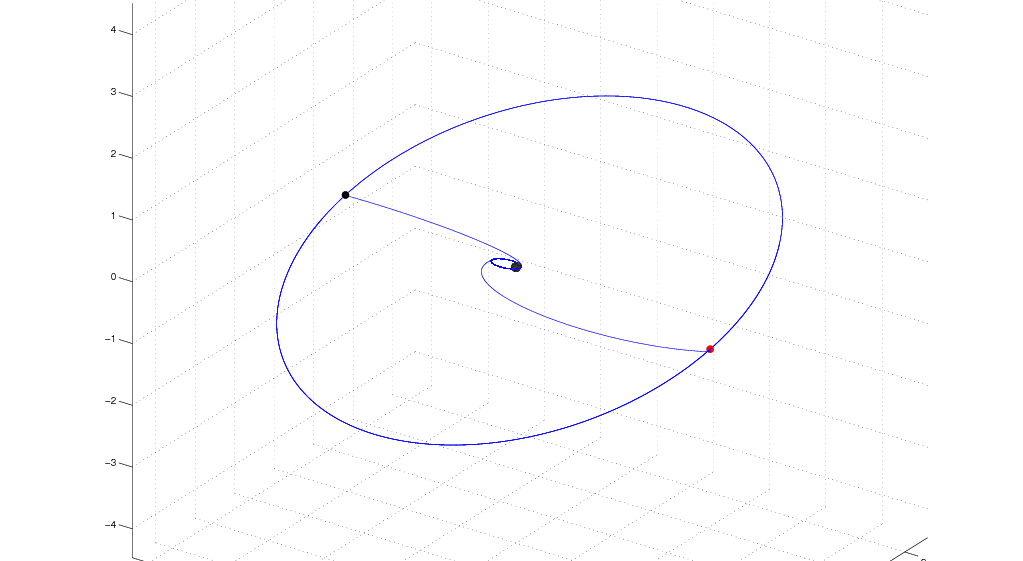
\includegraphics[width=\textwidth]{orbits.png}
  \caption{This graphic depicts the orbit of the satellite before its
    rockets are fired (inner orbit), the orbit of the moon (outer orbit),
    and the potential impact points as well as estimated trajectories of
    the satellite (the code for which is not included).}
  \label{fig:orbits}
\end{figure} 

\begin{figure}[H]\centering
  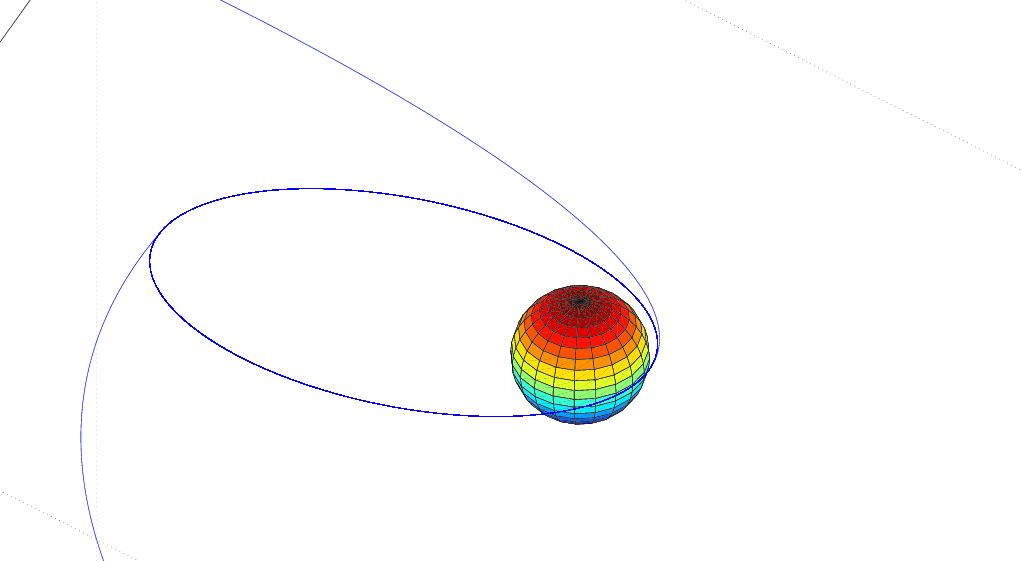
\includegraphics[width=\textwidth]{satorbit.png}
  \caption{Same as Figure.\ref{fig:orbits}, but zoomed in on the earth
    and satellite.}
  \label{fig:satorbit}
\end{figure} 

\noindent
The function for the equation of motion is at the end of the orbits script:

\begin{verbatim}
  % Equation of motion as a function of time and a position vector
% and velocity vector
function dwdt = eom(t,w)
  x=w(1); y=w(2); z=w(3);
  vx=w(4); vy=w(5); vz=w(6);
  r = sqrt(x^2+y^2+z^2);
  dwdt = [vx;vy;vz;-mu*x/r^3;-mu*y/r^3;-mu*z/r^3];
end
\end{verbatim}

\subsection{Other Functions}

\noindent
The function to process the moon data:

\begin{verbatim}
function [rp,vp,perigee,apogee] = moondata(file,grav_par)

% Converts degrees to radians
radians = @ (degrees) degrees*pi/180;

% Reads a csv and makes it an array
moondata = csvread(file);

% Stores the perigee and apogee and where they happen
[perigee,pind] = min(moondata(:,8));
[apogee,aind] = max(moondata(:,8));

% Stores the ra and dec at perigee and apogee
[ra_p,dec_p] = radec(pind);
[ra_a,dec_a] = radec(aind);

% Makes the position vectors at perigee and apogee. I admit this
% should be one function
rp = perigee * ...
     [cos(ra_p)*cos(dec_p), sin(ra_p)*cos(dec_p), sin(dec_p)];
ra = apogee * ...
     [cos(ra_a)*cos(dec_a), sin(ra_a)*cos(dec_a), sin(dec_a)];

% Crosses the position vectors at perigee and apogee to find a
% vector normal to the moon's plane
m = cross(rp,ra)./(norm(cross(rp,ra)));

% Finds velocity when moon is at perigee
vp = sqrt(2*grav_par*apogee/(perigee*(apogee+perigee))) * ...
     (cross(m,rp)/perigee);

% Function that outputs the ra and dec in radians for a given index
% of moondata.csv
function [ra,dec] = radec(index)
  % Stores the ra and dec in the file as some variables
  ra_deg = moondata(index,1:3);
  dec_deg = moondata(index,4:7)*moondata(index,4);

  % Converts ra_deg first to decimal degrees
  ra = ra_deg(1)*(360/24) + ...
       ra_deg(2)*360/(24*60) + ...
       ra_deg(3)*60/(24*60*60);
  % Then to radians and stores it as the output of the function
  ra = radians(ra);

  % Converts dec values in the file to decimal degrees then radians
  % and stores it as the second output of the function
  dec = dec_deg(2) + dec_deg(3)/60 + dec_deg(4)/(60*60);
  dec = radians(dec);
end
\end{verbatim}

\noindent
The function to find the initial conditions of the satellite:

\begin{verbatim}
  function [rp,vp,normalvector] =
satellite(inc,peri_alt,apo_alt,arg,long,rb,grav_par)

% Converts radians to degrees
radians = @ (degrees) degrees*pi/180;

% Converts the inclination, argument, and longitude to radians
inc = radians(inc);
arg = radians(arg);
long = radians(long);

% Adds the radius of the body its orbiting--earth
peri_alt = peri_alt + rb;
apo_alt = apo_alt + rb;

% Finds the initial position
rp = (peri_alt) * ...
     [ (cos(arg)*cos(long)-sin(arg)*sin(long)*cos(inc)), ...
       (cos(arg)*sin(long)+sin(arg)*cos(long)*cos(inc)), ...
       (sin(arg)*sin(inc)) ];

% Finds the initial velocity
vp = sqrt(2*grav_par*apo_alt/(peri_alt*(apo_alt+peri_alt))) * ...
     [ -(sin(arg)*cos(long)+cos(arg)*sin(long)*cos(inc)), ...
     (cos(arg)*cos(long)*cos(inc)-sin(arg)*sin(long)), ...
     (cos(arg)*sin(inc)) ];

% Finds the normal vector
normalvector = [sin(long)*sin(inc), -cos(long)*sin(inc), cos(inc)];
\end{verbatim}

\subsection{Graphs and Other Data}

A block of code in the \verb[orbits[ script produces the graphs
required as well as outputting the time it takes for the moon to orbit
the earth.

\begin{verbatim}
% Velocity of satellite while in orbit
v_sat = w_satvals(:,4:6);
% Speed of satellite while in orbit
speed_sat =
(w_satvals(:,4).^2+w_satvals(:,5).^2+w_satvals(:,6).^2).^.5;
% Position vector of satellite while in orbit
r_sat = w_satvals(:,1:3);
% Distance to center of eartch of satellite while in orbit
d_sat = (w_satvals(:,1).^2+w_satvals(:,2).^2+w_satvals(:,3).^2).^.5;
% Total energy of satellite while in orbit
e_sat = .5 * speed_sat.^2 - mu./d_sat;

% Graphs the total energy per unit mass of the satellite
figure;
plot(t_sat,e_sat);
title('Graph of total energy of satelite per unit mass');
axis([0 time*2 min(e_sat) max(e_sat)]);

% Finds the angular momentum per unit mass of the satellite while
% in orbit by taking the cross product of its position vector and
% velocity vector at every time index
for i = 1:length(t_sat);
  L_sat(i) = norm(cross(r_sat(i,:),v_sat(i,:)));
end

% Graphs angular momentum per unit mass of the satellite while in
% orbit
figure;
plot(t_sat,L_sat);
title('Graph of angular momentum of satellite per unit mass');
axis([0 time*2 min(L_sat) max(L_sat)]);

% Prints the perigee of the moon
peri_moon
% Prints the apogee of the moon
apo_moon

% Displays the number of days that it takes for the moon to go
% around the earth
moontime = (t_impmoon(3) - t_impmoon(1))/60/60/24;
disp(sprintf('Moon orbits in %d days',moontime));
\end{verbatim}

\noindent
The output of that is Figures.\ref{fig:energy},\ref{fig:momentum}

\begin{figure}[H]\centering
  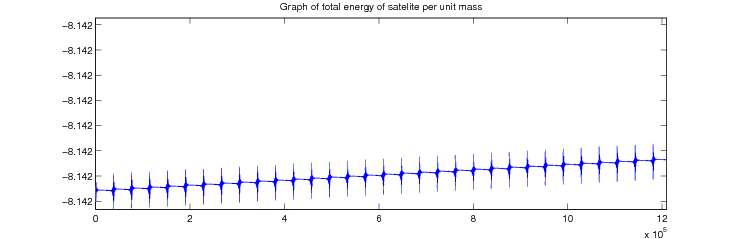
\includegraphics[width=\textwidth]{satelliteenergy.png}
  \caption{The total energy of the satellite divided by its mass as a
    function of seconds.}
  \label{fig:energy}
\end{figure}

\begin{figure}[H]\centering
  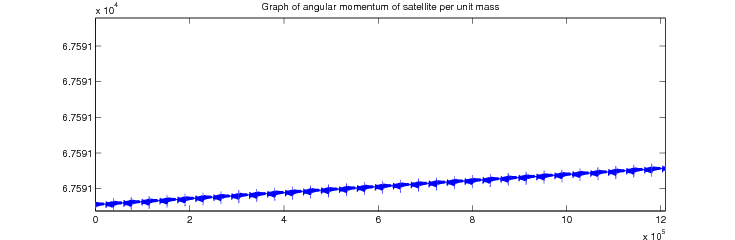
\includegraphics[width=\textwidth]{satellitemomentum.png}
  \caption{The angular momentum of the satellite as a function of
    seconds.}
  \label{fig:momentum}
\end{figure}

\noindent
And, of course:
\begin{verbatim}
peri_moon =

   3.5658e+05


apo_moon =

   4.0666e+05

Moon orbits in 2.715414e+01 days
\end{verbatim}

\end{document}
